\documentclass[12pt]{article}
\usepackage[utf8]{inputenc}
\usepackage[cm]{fullpage}
\usepackage[]{graphicx}
\usepackage{setspace}
\usepackage{calc}

\newlength{\remaining}
\newcommand{\titleline}[1]{%
\setlength{\remaining}{\textwidth-\widthof{\textsc{#1}}}
\noindent\underline{\textsc{#1}\hspace*{\remaining}}\par}



\title{ 
\includegraphics[scale=.25]{images/Contra-Logo.png} }
\author{Aleksandr Khavarovskiy, \\ Daniil Kernazhytski}

\usepackage{float}
\floatstyle{boxed} 
\restylefloat{figure}

\usepackage{graphicx}
\usepackage{sidecap}

\usepackage{graphicx}
\newcommand{\species}[1]{\textit{#1} sp.}

\begin{document}

\maketitle
\section*{\titleline{Abstract} } 
Contra is a single player or co-op, side scrolling platformer in which the goal is to eliminate various enemies using various weapons to progress onto the next level. Our adaptation will be a co-op arcade version with the same general mechanics as the original and with the added benefit of networking.  The arcade version of the game will entail two soldiers who will be fighting off hordes of enemies that charge at the players in waves. The biggest difference being that the arcade version will take place on a single limited stage that will incorporate side mechanics. To goal of the game will require the two soldiers to survive as many hordes of enemies while eliminating them to score points in an  attempt to reach top of the scoreboard. The players will navigate platforms and fire projectiles in attempts to eliminate enemy AI. We plan to have power-ups that are dropped randomly by enemies or we will incorporate a system in which the players will be able to use earned points to purchase these powerups.  These power-ups will include various weapons and player attribute boosts, such as, speed, lives and weapon firing speed. We believe this will be an interesting approach because, it takes the arcade mechanics and art style of 80’s video games and combines them with the very successful survival mode similar to Nazi Zombies. A game mode originally developed for the modern Call of Duty franchise.

\newpage
\section*{\titleline{UI} } 
The games user interface will be as closely resembled to the original game as possible with a few possible additions or removals where we see fit. The original UI style of the game embedded the scoring system and live counter into the corner of the playing field. 
\begin{center}
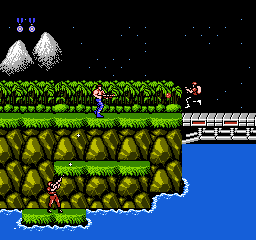
\includegraphics[scale=1]{images/Contra.png} 
\end{center}

\section*{\titleline{Architecture} } 
For our networking component we plan to use a peer to peer system. The will use the dumb client model for our implementation. We will use TCP as our means of network communication. This will ensure reliability of information but may have issues with consistencies over long distance communication. The client will issue commands to move, jump or fire. The server will respond with the information pertaining to the entities on the server and the client will render these entities accordingly. The server will have to send entity position, velocity and state. Entities will primarily include players, enemies and projectiles. To ensure consistency we will use the server delta as the time standard for the client. This will ensure that the client is updated in the same increments as the server.

\section*{\titleline{Development Strategy} }
The project will be started essentially from scratch. The slick2D engine and the accompanying jig library will be used for loading and displaying the graphics on to the screen. The entire project will thus pe written in Java. We will also be using the IntelliJ IDEA programming environment as it is far superior and more pleasant to work in compared to Eclipse.

\begin{itemize}
	\item Alex: will focus on the networking side of things as well as level design 
	\item Daniil: will focus on animations, collisions and game logic. IE making the game work.
\end{itemize}

\section*{\titleline{High Bar} } 

\begin{itemize}
	\item Destructible Bridges and water terrain.
	\item Water terrain allows for restricted movement (no jumping), but is otherwise freely accessible. 
 	\item Additional single player mode.
\end{itemize}

\section*{\titleline{Low Bar} }
The low bar goal represents more of a Pac-Man style game with a different themes, enemies and abilities. 
\begin{itemize}
	\item Game menu with title screen.
	\item Include the Ability for Coop mode (2 players) to play over a network 
	\item Have infinite waves of enemies attack the players
 	\item The Game looks and feels like the NES Contra 
	\item Gun Power-ups
\end{itemize} 

\end{document}
